\documentclass[11pt]{article}

\usepackage[paperwidth=8.5in, paperheight=11in, top=1in, bottom=1in, right=.75in, left=.75in]{geometry}
\usepackage{wrapfig}
\usepackage{graphicx}
\usepackage{listings}
<<<<<<< HEAD
\usepackage{pgfplots} 
\usepackage{pgfplotstable}
\pgfplotsset{compat=1.5}
=======
\usepackage[table]{xcolor}
>>>>>>> origin/master

\title{Project 3}
\author{Cera Olson\\Jacob Mastel\\Robert Erick}
\date{\today}

\newcommand{\e}[1]{\ensuremath{\times 10^{#1}}}

\lstset{
	tabsize=4
}

\pagenumbering{gobble}
	
\begin{document}
	\maketitle\textbf{Total Calories:} \$ \\
\textbf{Total Cost:} \$
	\clearpage
\section*{Question 1}
	\section*{Question 2}
	%
\section{Part A}
One alternative to the least squares line is the Least Absolute Deviations (LAD). Formulate a linear program whose optimal solution minimizes the sum of the absolute deviations of the data from the line. That is formulate 
\begin{center} $ min  \sum_{i=1}^{n} |y_{i} - (a_{1}x_{i} + a_{0})|$ \end{center} 
as an LP and solve for the $a_0$ and $a_1$ that minimize the sum of absolute deviations.

\subsection{i: Write the linear program for the general problem written as an objective and set of constraints}
The goal is to minimize $ min  \sum_{i=1}^{n} |y_{i} - (a_{1}x_{i} + a_{0})|$. In order to create an objective, we drop the sum and set it equal to $z_i$ for all values $i = 1,...,n$. We can reduce that by dropping the absolute values and set it as an inequality.
\begin{center} $-z_{i} \leq y_{i} - (a_{1}x_{i} + a_{0}) \leq z_{i}$  \end{center}
After that it gets simplified down to the following objectives and constraints. 

\begin{center} $ y_{i} - (a_{1}x_{i} + a_{0}) \leq z_{i}$  for all values $i = 1,...,n$\end{center}
\begin{center} $ y_{i} - (a_{1}x_{i} + a_{0}) \geq -z_{i}$  for all values $i = 1,...,n$\end{center}

\subsection{ii: Use the linear program to find the LAD regression line for the data set $(x,y) = { (1,5), (1, 3), (2, 13), ( 3, 8), (4,10), ( 5, 14), (6, 18) }$
What was the sum of absolute deviations?}

The absolute deviation is calculated by taking the least squares values for y and finding the difference between that and the calculated actual value of y using the data. See the chart below. The trendline has an equation of $y = 2.315x + 2.875$

\begin{table}[ht]
\caption{Part A (ii)}
\centering
\begin{tabular}{c | c | c | c | c}
\hline\hline
x & y: Data Points & Trendline & Differences & Squared \\ [0.5ex] % inserts table %heading
\hline
1 & 5 & 3.93 & 1.07 & 1.15 \\
1 & 3 & 3.93 & 0.93 & 0.87 \\
2 & 13 & 5.99 & 7.01 & 49\\
3 & 8 & 8.07 & 0.07 & 0.01 \\
4 & 10 & 10.14 & 0.14 & 0.02 \\
5 & 14 & 12.21 & 1.79 & 3.2 \\
6 & 18 & 14.29 & 3.72 & 13.84 \\ [1ex]
\hline
\end{tabular}
\label{table:nonlin}
\end{table}

Based on the chart above, the sum of the absolute deviations is 14.73.

\subsection{iii: Plot the points and graph your LAD line and the least squares line. Comment.}
The value for point 2 appears to be an outlier. The value of the data point at x = 2 falls outside the line of best fit the most. 

\begin{figure}[h] %  figure placement: here, top, bottom, or page
   \centering
   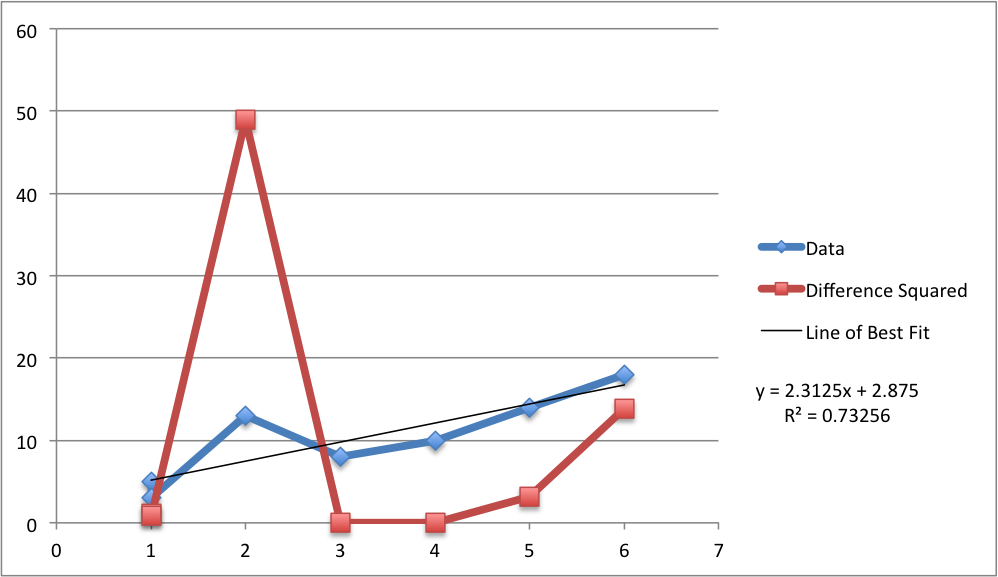
\includegraphics[width=\textwidth,height=\textheight,keepaspectratio]{Q3PAiii.png} 
   \caption{example caption}
   \label{fig:example}
\end{figure}
%\begin{tikzpicture}
%\begin{axis}[
%    title={Part A ii},
%    xlabel={x values},
%    ylabel={y values},
%    xmin=0, xmax=7,
%    ymin=0, ymax=20,
%    xtick={0,1, 2, 3, 4, 5, 6},
%    ytick={0,4, 8, 12, 16, 20},
%    legend pos=north west,
%    ymajorgrids=true,
%    grid style=dashed,
%]
%    \addplot[color=blue,
%    mark=square] table{
%        X Y
%        1 5
%        1 3
%        2 13
%        3 8
%        4 10
%        5 14
%        6 18 };
%    \addlegendentry{True Data}
%    \addplot table[
%        y={create col/linear regression={y=Y}}] % compute a linear regression from the input table
%    {
%        X Y
%        1 5
%        1 3
%        2 13
%        3 8
%        4 10
%        5 14
%        6 18};
%    \addlegendentry{%
%        $\pgfmathprintnumber{\pgfplotstableregressiona} \cdot x
%        \pgfmathprintnumber[print sign]{\pgfplotstableregressionb}$};
%
%\end{axis}
%\end{tikzpicture}

\section{Part B}
Another alternative to the least squares method is to find a line that minimizes of the maximum absolute deviation (MMAD). That is formulate
\begin{center} $min\  max_{i}\  | y_{i}  - (a_{1}x_{i} + a_{0}) |$ \end{center}
as an LP.

\subsection{i: Write the linear program for the general problem written as an objective and set of constraints}
Following the same procedures as in Part A, set the equation equal to z and try to minimize z for all values $i = 1, ... , n$. The resulting equations are:
\begin{center} $ y_{i} - (a_{1}x_{i} + a_{0}) \geq z_{i}$  for all values $i = 1,...,n$\end{center}
\begin{center} $ y_{i} - (a_{1}x_{i} + a_{0}) \leq -z_{i}$  for all values $i = 1,...,n$\end{center}
It is important to note that these are opposite of the solutions as found in part A.

\subsection{ii: Use the linear program to find the MMAD regression line for the data set $(x,y) = { (1,5), (1, 3), (2, 13), ( 3, 8), (4,10), ( 5, 14), (6, 18) }$ What was the min of the max absolute deviations?}
Minimize z subject to $ z \geq max_{i}\ |{y_{i} - (a_{1}x_{i} + a_{0})|}$



\subsection{iii: Plot the points and graph the MMAD line and the least squares line. Compare.}


\subsection{iv: Can you create a data set for which all three methods of regression (least squares, LAD, MMAD)
compute the same line.}
The only set that could have the same result is the empty set or a set of zero values. All three methods use different methodologies to calculate the line of best fit. They all use either minimization, maximization, or a combination there of, and as such, there will be minute differences between the calculations of the regression. 


\section{Part C}
Multiple Linear Regression. Generalize the simple linear regression model to allow for two independent variables ($x_{1}$ and $x_{2}$).
$?? = ??_{2} ??_{2} + ??_{1} ??_{1} + ??_{0}$ ,
The model is called multiple linear not because the result is a line but because all variables are 1st degree. Extend the techniques from Part A to find the least absolute deviations regression equation. Use linear programming to fit a LAD multiple linear regression model to the data set below:
\begin{table}[ht]
\centering
\begin{tabular}{| c | c | c |}
\hline
$x_{1}$ & $x_{2}$ & y \\ [0.5ex] % inserts table %heading
\hline
1 & 1 & 5 \\
1 & 2 & 9  \\
2 & 2 & 12 \\
0 & 1 & 3  \\
0 & 0 & 0  \\
1 & 3 & 11 \\ [1ex]
\hline
\end{tabular}
\end{table}

Solving for $a_{0}$, $a_{1}$, and $a_{2}$ using a system of equations and the values in the table above. Using the above values, $a_{0}$ must be 0. It is the only way $x_{1}$ and $x_{2}$ could be zero if y is 0. The result is that $a_{2}$ equals 3. The final value, $a_{1}$, is 2 or 3 depending on the data points you use to calculate them.  Using LAD, we minimize the values. making $a_{1} = 2$.
\\
The final estimation is $y = 3\times x_{2} + 2\times x_{1}$.

\end{document}